%%%%%%%%%%%%%%%%%%%%%%%%%%%%%%%%%%%%%%%%%
% Simple Sectioned Essay Template
% LaTeX Template
%
% This template has been downloaded from:
% http://www.latextemplates.com
%
% Note:
% The \lipsum[#] commands throughout this template generate dummy text
% to fill the template out. These commands should all be removed when 
% writing essay content.
%
%%%%%%%%%%%%%%%%%%%%%%%%%%%%%%%%%%%%%%%%%

%----------------------------------------------------------------------------------------
%	PACKAGES AND OTHER DOCUMENT CONFIGURATIONS
%----------------------------------------------------------------------------------------

\documentclass[12pt]{article} % Default font size is 12pt, it can be changed here

\usepackage{geometry} % Required to change the page size to A4

\usepackage{titlesec}

\usepackage{framed}

\usepackage[hidelinks]{hyperref}

\usepackage[utf8]{inputenc} % Use this package to enable the use of special norwegian characters (æ, æ, å)

\geometry{a4paper} % Set the page size to be A4 as opposed to the default US Letter

\usepackage{graphicx} % Required for including pictures

\usepackage{float} % Allows putting an [H] in \begin{figure} to specify the exact location of the figure
\usepackage{wrapfig} % Allows in-line images such as the example fish picture

\usepackage{cite}

\usepackage{url}

\usepackage{pdfpages}

\usepackage{supertabular} % Used for tables

\usepackage{tocbibind}

\usepackage[parfill]{parskip} % Newline without indent

\usepackage{lipsum} % Used for inserting dummy 'Lorem ipsum' text into the template

\usepackage[T1]{fontenc}

\usepackage{array}
\linespread{1.2} % Line spacing

\usepackage{xcolor,colortbl}

\setcounter{secnumdepth}{4}
%\setcounter{section}{1}

%\setlength\parindent{0pt} % Uncomment to remove all indentation from paragraphs

\graphicspath{./graphics/} % Specifies the directory where pictures are stored

\setcounter{tocdepth}{5} %to make it appears in TOC
%\setcounter{secnumdepth}{5} %to make it numbered

\titleformat*{\section}{\LARGE\bfseries}
\titleformat*{\subsection}{\Large\bfseries}
\titleformat*{\subsubsection}{\large\bfseries}
\titleformat*{\paragraph}{\footnotesize\bfseries}
%\titleformat*{\subparagraph}{\large\bfseries}

\begin{document}
%----------------------------------------------------------------------------------------
%	TITLE PAGE
%----------------------------------------------------------------------------------------

\begin{titlepage}

\newcommand{\HRule}{\rule{\linewidth}{0.5mm}} % Defines a new command for the horizontal lines, change thickness here

\center % Center everything on the page

\textsc{\LARGE Gjøvik University College}\\[0.5cm] % Name of your university/college

\includegraphics[width=90px, height=90px]{graphics/google_tv_logo}\\[0.8cm] % Include a department/university logo - this will require the graphicx package 403x403px
\textsc{\Large Software Engineering}\\[0.5cm] % Major heading such as course name
\textsc{\large Group Project}\\[0.5cm] % Minor heading such as course title

\HRule \\[0.4cm]
{ \huge \bfseries EpisodeGuide}\\[0.4cm] % Title of your document
\HRule \\[1.5cm]

\begin{minipage}{0.44\textwidth}
\begin{flushleft} \large
%\emph{Authors:}\\
Victor \textsc{Rudolfsson} - 120912\\ % Your name
Tommy \textsc{B. Ingdal} - 120913\\ % Your name
Halvor \textsc{Thoresen} - 120915\\ % Your name
\end{flushleft}
\end{minipage}

\vfill % Fill rest of the page with empty lines
{\large \today}\\[3cm] % Date, change the \today to a set date if you want to be precise

\end{titlepage}

%----------------------------------------------------------------------------------------
%	TABLE OF CONTENTS
%----------------------------------------------------------------------------------------
\tableofcontents % Include a table of contents
\newpage % Begins the essay on a new page instead of on the same page as the table of contents 

%----------------------------------------------------------------------------------------
%	PART 1
%----------------------------------------------------------------------------------------
\section{Project Plan}
%----------------------------------------------------------------------------------------
%	goals_and_frameworks
%----------------------------------------------------------------------------------------
\subsection{Goals and frameworks}
\subsubsection{Background}
FrostByte, a fictional company,  is a company specializing in informative web solutions for everything related to TV-shows.
The company has previously had a decent product which covered their basic needs, but has recently been met with increasing competition. Because of this, they’ve decided to further develop their product and give their existing and new users a completely new product with increased functionality which they hope will give them a competitive edge.

\subsubsection{Brief description of product}
The final product should present users with a grid of all TV-shows known to man. Users should be able to browse through TV-shows, view details about them, as well as details about every individual episode.
Users should also be able to create user accounts, to allow them to log in and access otherwise unavailable features. Such features may include e.g \textit{following} specific TV-shows, generating a calendar view of upcoming episode release dates for followed shows, and mobile push notifications.

It goes without saying that users should be able to search for shows, actors and/or episodes, and filter shows using a variety of different categories such as channel it was originally broadcast on, who acts in it, or what rating it has been given on international sites such as IMDb.

It should be possible to assign users roles, such as Administrator, Moderator, Grand Suncrusher or Newly Registered through the administrator interface. An administrator should also be able to \textit{force} an update of the contents in the database (something which should otherwise be done in regular intervals automagically). 

The design needs to be responsive, as to adapt well for hand held devices.

\subsubsection{Goals}

\paragraph{Expected results}~\\
It’s expected that the finished product should be able to:\\
       -    register new users\\
       -    allow users to stay up-to-date with new and old TV-shows\\
       -    suggest new TV-shows based on the users preferences\\
       -    distribute e-mail to all users when there are significant news (news letters)\\
       -    export TV-schedule to an existing calendar (iOS, Android, WP8)\\
       -    offer advertising space to other companies\\
       -    allow users to pay for additional functionality\\
       -    the platform should also be easily managed and maintained. 

\paragraph{Expected impact}~\\
By developing this system, the company expects the following effects:\\
      -    Increased publicity\\
      -    By utilizing new technology and functionality, become leading within their niched market\\
      -    30\% increased profit the first year\\
      -    40\% more visitors

\subsubsection{Frameworks}
The project is executed and delivered within the provided framework.

\paragraph{Legal framework}

The finished system may not violate the Norwegian Personal Data Act §§8-17

\paragraph{Technological frameworks}~\\
The system should have gone through a thorough security audit before being handed over, to ensure the safety of users’ information.

\paragraph{Budget and time frame}~\\
FrostByte has stated they want the system up and running by 15. dec. 2014. Furthermore, the project has a budget of 3.5 million NOK.
 % Includes the file that contains the introduction

%----------------------------------------------------------------------------------------
%	scope
%----------------------------------------------------------------------------------------
\subsection{Scope}
\subsubsection{Definitions and limits}

FrostByte is a company that currently has a large pool of information about old and current TV-shows, and has for a long time had a web interface to present this information to its users.\\
As a result of increased competition from other actors on the market, and a strong need for better functionality, a new system titled EpisodeGuide will be developed.

The project will eventually result in a robust system allowing users to register accounts, which will provide them with functionality exclusive to registered users.\\
It’ll also be possible to provide users with premium functionality for a small monthly fee.\\
Administrating the system and distributing new information to the users should be made simple and smooth, by utilizing new and innovative technology and services. 

FrostByte already has a platform / web-interface built on an old but working code base, and they’d like to see some of the old functionality migrated to the new system.\\
As branches of the platform, mobile applications should be developed to allow for communication with the platforms API. The mobile applications should be released primarily for iOS, Android and Windows Phone.

From a security perspective, because sensitive data such as credit card information and personal user data may be stored, it’s important that this data is treated, transmitted and stored in a secure manner. Because of this, FrostByte has entered a partnership with MasterCard/VISA for secure payment solutions.
 % Includes the file that contains the introduction

%----------------------------------------------------------------------------------------
%	project_organization
%----------------------------------------------------------------------------------------
\subsection{Project organization}
\subsubsection{Resources and responsibilities}
The development-company is rather small, with only 7 employees. No previous projects require maintenance, and thus 100\% of the available resources are allocated to develop the product for FrostByte.
Part of the tasks differ significantly from one another, so to make development as effective as possible over a small group of employees, the workload is split into tasks and distributed over the team.


The development team is split into the following groups:\\
\begin{itemize}
\item One project owner / employer\\
\item One SCRUM master\\
\item Two developers working on backend\\
\item Two developers working on solutions for handheld devices\\
\item One developer working on design
\end{itemize}

All employees are experienced and competent within these fields, and workload can thus be delegated rather flexibly if required.

\subsubsection{Miscellaneous roles and employment}

The development team does not have enough resources to perform thorough testing of the system, and thus an external user group will be established which will be given access to the system whilst it’s still under development. This will provide the development team with enough useful feedback and a good overview of bugs and missing features in the platform.\\
This user group will consist of volunteering invidiuals who’ve shown an interest in the project through various communication channels. The group will be as diverse as possible, with people of different background and expertise (or lack thereof), which should lead to a large variety of different perspectives and thus, more varied feedback.
A new version should be rolled out once every 2 weeks into the testing environment.

Security is an important focus for FrostByte, and an external security audit-team will therefore be brought in to make sure all development is done with security as part of the development life cycle. This will also help improving and maintaining the trust-relation between the company and its users.

\subsubsection{Choice of development methodology}
\paragraph{Daily and weekly SCRUM meetings}~\\
Every day, the developers will be given an overview of the goals for the day. Problems and challenges can be discussed and space will be given to make adjustments if needed.~\\

Every second week, at the end of each sprint, the developers should engage in a combined sprint review and sprint retrospective meeting, where they shall present a short overview of which tasks have been completed and what problems and challenges have arisen since the beginning of the last sprint.

Because these meetings are common to all developers, time will be allocated at the end of the meeting to allow for a short discussion of the potential issues and challenges.

\paragraph{Meetings with product owner}~\\
Every other week, a meeting between the product owner and the development team will be held to ensure an active dialog. During this meeting it will be possible to suggest adjustments and changes of the product, and for the product owner to be given a brief report of the current development state.
 % Includes the file that contains the introduction

%----------------------------------------------------------------------------------------
%	planning_monitoring_and_reporting
%----------------------------------------------------------------------------------------
\subsection{Planning, monitoring and reporting}
\subsubsection{Discussion of overall development method}
The development company consists of six skilled people with broad expertise within web-technology and development. The project consists of a variety of different development methods and the complexity is rather high; thus it is expected that development will take around 10 months to reach completion.\\
With such a system, it’s highly plausible the product owner change their mind regularly as a result of feedback from users. The project builds on an existing system and existing users, and thus is not considered a high risk factor.\\

SCRUM has been chosen as the development methodology, mainly because a sprint time of 14 days will help in providing incremental revisions that can be tested by both product owner and user testing group. This is especially important because of the risk of changes being made to the project. The project requirements may be modified according to product owner’s and users’ feedback, which is why it’s important to continuously review previously completed functionality to improve or make changes to the code.
The system is developed by a relatively small team, something which requires each employee to complete their respective tasks within the given time frame. With SCRUM sprints it will be simpler to measure success and workload to make sure a consistent and stable workflow is maintained.
 % Includes the file that contains the introduction

%----------------------------------------------------------------------------------------
%	risk_analysis
%----------------------------------------------------------------------------------------
\subsection{Risk analysis}

The level of risk is calculated by multiplying these factors, probability and impact, with one another. After calculating the risk, a number between 1-16 indicates the risk level, where 1 is the lowest possible risk and 16 is the highest possible risk. To more easily see what is an actual risk, we have defined an acceptable risk level of 4. Everything with a risk level below 4 is considered acceptable risk.

\subsubsection{Identify and Analyze project risks}
\begin{tabular}{|l|l|l|l|}
\hline
	Description 							& Probability & Impact 	& Risk level \\
\hline Loss of source code 						& 1		& 4 		& \cellcolor{green} 4 \\
\hline Project exceeds budget 					& 2 		& 3		& \cellcolor{orange} 6 \\
\hline Sudden change of requirement specification 		& 3 		& 2 		& \cellcolor{orange} 6 \\
\hline Project exceeds timeframe 				& 2 		& 2 		& \cellcolor{green} 4 \\
\hline Project cancellation 						& 1 		& 4		& \cellcolor{green} 4 \\
\hline Loss of communication between dev. team and users 	& 4 		& 2 		& \cellcolor{red} 8 \\
\hline
\end{tabular}
Fig - Risk table

\subsubsection{Plan for managing the most critical risks}

\paragraph{Project exceeds budget}~\\
Risk can be reduced by performing a monthly review of expenses, and by establishing a financial budget for the development timeframe.

\paragraph{Sudden modification of requirement specification}~\\
By maintaining a good and active dialogue between product owner and development team, preferably once every other week, this risk can be reduced.
Additionally, a thorough meeting will be held between product owner and development team led by the scrum master before the first sprint starts, to make sure all requirements and requests have been presented and considered..

\paragraph{Loss of communication between development team and users}~\\
This risk can be reduced by actively utilizing the user group. As soon as new functionality is complete it should be published for testing by the user group, as to allow them to continuously provide constructive feedback on the latest implemented features.
 % Includes the file that contains the introduction

%----------------------------------------------------------------------------------------
%	implementation
%----------------------------------------------------------------------------------------
\subsection{Implementation}
\subsubsection{Decision deadlines}
01. mar - Will the project be developed?\\
15. mai - Use of technology

\subsubsection{Milestones}
25. feb - Project plan finalized.\\
21. mar - Requirement specification finalized.\\
25. apr - Design-plan finalized.\\
15. may - Complete project report done.\\
15. dec - Evaluation report done.\\
15. dec - System fully developed.\\


\subsubsection{Timeframe}

\hspace*{-1.2in}
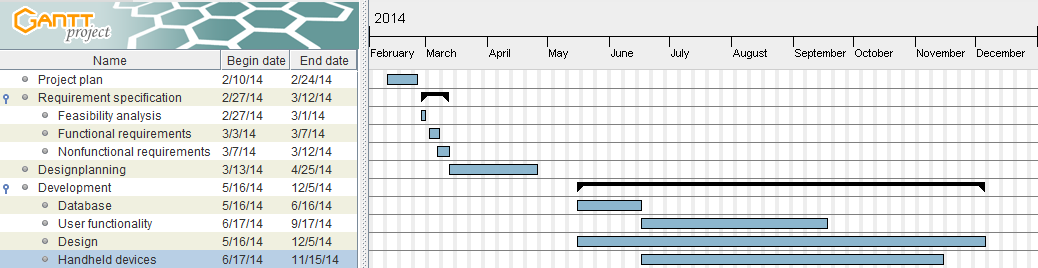
\includegraphics[scale=0.75]{graphics/gantt}
 % Includes the file that contains the introduction

%----------------------------------------------------------------------------------------
%	DEL II
%----------------------------------------------------------------------------------------
\newpage
\section{Requirement Specification}

\subsection{Use Case Diagram}
\begin{figure}[h]
\setlength\fboxsep{0pt}
\setlength\fboxrule{0.2pt}
\fbox{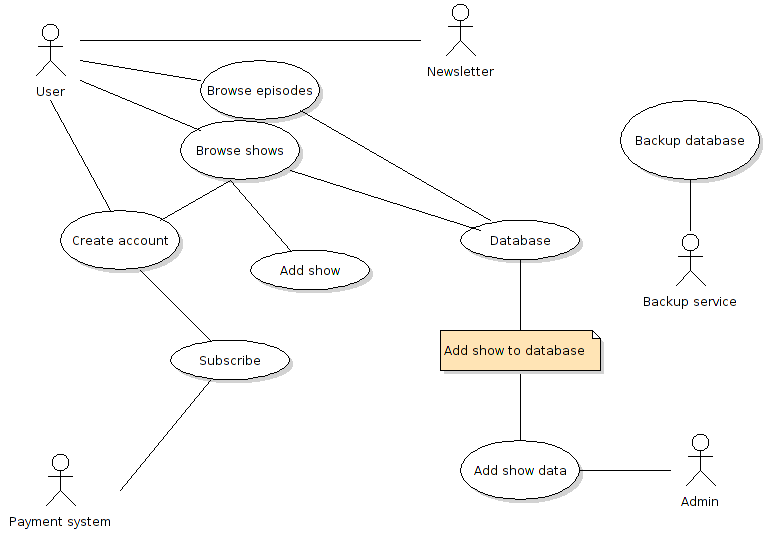
\includegraphics[scale=0.6]{graphics/usecasediagram.png}}
\caption{Use Case Diagram}
\end{figure}

\subsubsection{Comments on Use Case Diagram}
In the use case diagram we have five entities which make up the flow of the application.
The user, and also the main entity, is the one that interacts with most of the parts of the application (exluding: backup system and administration).
The administrator is the entity that adds data to the database (ie. new shows and/or episodes) or sends out newsletter.
\\
In our model we have one external entity; the payment system. This system allows the users to upgrade their account and pay their subscription fee directly via the web application.
The application communicates with the payment backend (ie. Visa/Mastercard) over a secure channel.\\
The backup system, as of today, only have one job; on regular intervals, make a backup of all the user accounts and associated data.


\subsection{High level Use Case Descriptions}

\begin{framed}
\begin{tabular}{ l p{11cm}}
  \textbf{Use Case} & Add show data \\
  \textbf{Entity} & Admin \\
  \textbf{Goal} & Keep the database up to date\\
  \textbf{Description} & The administrator make sure the database is up to date with all the newest show and episode data. \\
\end{tabular}
\end{framed}

\begin{framed}
\begin{tabular}{ l p{11cm}}
  \textbf{Use Case} & Backup \\
  \textbf{Entity} & Backup, Admin \\
  \textbf{Goal} & Make a copy of the database and keep the database safe.\\
  \textbf{Description} & The database will make a backup on regular intervals, but the administrator can initiate a backup process whenever he wants. \\
\end{tabular}
\end{framed}

\begin{framed}
\begin{tabular}{ l p{11cm}}
  \textbf{Use Case} & Newsletter \\
  \textbf{Entity} & Admin \\
  \textbf{Goal} & Sends newsletters to user. \\
  \textbf{Description} & The administrator can, through the administration page, send newsletter/emails to his users. \\
\end{tabular}
\end{framed}

\begin{framed}
\begin{tabular}{ l p{11cm}}
  \textbf{Use Case} & Subscribe \\
  \textbf{Entity} & User \\
  \textbf{Goal} & Subscribe to a member-only service.\\
  \textbf{Description} & After a user has created an account, it is possible to subscribe to member-only services. The user will be prompted to pay a subscription fee which will be handled by Visa/Mastercard. All the data transfered between the client/server is encrypted (uses SSL/TLS). \\
\end{tabular}
\end{framed}

\begin{framed}
\begin{tabular}{ l p{11cm}}
  \textbf{Use Case} & Browse \\
  \textbf{Entity} & User \\
  \textbf{Goal} & View information about tv shows.\\
  \textbf{Description} & A registered user, as well as a non-registerered user, can use the application to find information about shows and episodes by searching the database. \\
\end{tabular}
\end{framed}
\subsection{Detailed use case}

\begin{tabular}{|p{16.5cm}|}
\hline
\textbf{Name:} Subscribe \vline   \textbf{ Actors:} User | Payment system \\ \hline
\textbf{Pre-condition:} User has created account. Connection with payment system is up.\\ \hline
\textbf{Post-condition:} Payment system will either accept or decline the User information input, \\and then send the appropriate response to database. \\ \hline
\textbf{Trigger: } User wants to upgrade the account to a paid subscription. \\ \hline
\textbf{Event flow: }
\begin{enumerate}
	\item The user requests the subscription page.
	\item User fills out and submits the necessary payment information:
	\begin{enumerate}
		\item First and Last name
		\item Card number
		\item Expiration date
		\item Card Verification Value
	\end{enumerate}
	\item The information is encrypted and sent over a secure connection to the payment system.
	\item Payment system recieves and decrypts the information.
	\item Payment system executes the necesarry verifications and confirmations.
	\item The appropriate response is sent back to the user
\end{enumerate}
\\ \hline
\textbf{Event variation: }
\begin{enumerate}
	\item User has not created an account:
	\begin{enumerate}
 		\item The requested subscription page will not be displayed.
		\item The user will be sent to the create account page.
	\end{enumerate}
	\item User submits invalid information that does not fit the input template:
	\begin{enumerate}
 		\item The information will not be sent to the payment system.
		\item The subscription page will be reloaded and an error message will be displayed.
	\end{enumerate}
	\item  The payment system response is positive and the transaction went without problems:
	\begin{enumerate}
 		\item  The user's status is updated.
	\end{enumerate}
	\item  The payment system response is negative and the transaction did not go through:
	\begin{enumerate}
 		\item  An error message will be displayed and the process will be terminated.
		\item The subscription page will be reloaded for the user.
	\end{enumerate}
\end{enumerate}

\\ \hline
\end{tabular} 

\begin{tabular}{|p{16.5cm}|}
\hline
\textbf{Name:} Backup database \vline   \textbf{ Actors:} Backup service | Admin\\ \hline
\textbf{Pre-condition:} There is an already existing database.\\ \hline
\textbf{Post-condition:} A full backup of the database is created and stored separatly from the original \\ \hline
\textbf{Trigger: } The backup serive requests a backup on regular intervals | The admin manually requests a backup. \\ \hline
\textbf{Event flow: }
\begin{enumerate}
	\item Either the admin or the backup service requests to run a backup.
	\item The backup service checks if any changes had been made since last backup.
	\item The backup service checks if there is enough disk space for the backup to be written to disk.
	\item The backup service creates an exact copy of current database and stores to the appropriate disk with the current timestamp.
\end{enumerate}
\\ \hline
\textbf{Event variation: }
\begin{enumerate}
	\item No existing database can be found:
	\begin{enumerate}
 		\item The process will be terminated.
		\item An error message will be written to the log.
	\end{enumerate}
	\item No changes has been made:
	\begin{enumerate}
 		\item The process will be terminated.
	\end{enumerate}
	\item Not enough disk space to store backup:
	\begin{enumerate}
 		\item The process will be terminated.
		\item An error message will be written to the log.
	\end{enumerate}
	\item Not enough disk space to store backup:
	\begin{enumerate}
 		\item The process will be terminated.
		\item An error message will be written to the log.
		\item An email will be sent to the the appropriate administrator.
	\end{enumerate}
	\item Backup is interrupted mid-process:
	\begin{enumerate}
 		\item The process will be terminated.
		\item The files already written to disk will be removed.
		\item An error message will be written to the log.
	\end{enumerate}
\end{enumerate}

\\ \hline
\end{tabular} 
\subsection{Operational Requirements}

\subsubsection*{Usability}
\begin{itemize}
\item Navigation should be the first thing apart from the logo that the user spots in the system
\item It should be self-evident how to get to the desired part of a site (e.g., if user finds a show, it should be obvious how to get to a specific episode of that show)
\item Reloading the page should not be necessary for small tasks such as subscribing to a show
\item Signing up should not require more information from the user than is necessary, to encourage signing up and reduce amount of users who refrain from doing so
\item Sharing content from the site to social media should be simple and preferably done with a single click without bloating the front-end with unnecessary icons
\item The administrators should not need to re-learn everything. Since we are building this project on top of some existing code, the administrators should be able to do things the way they are used to.
\item The layout should be clean and minimalistic.
\end{itemize}

\subsubsection*{Availability}
\begin{itemize}
\item The application should have an uptime of at least 99\% (i.e. 24 hours/day, every day of the year) to be able to compete with other actors on the market, and to be able to provide a reliable API for mobile applications and potential third parties who may want to access data. 
\end{itemize}

\subsubsection*{Reliability}
\begin{itemize}
\item If a bug is discovered it should be patched as soon as possible. This should not take more than 48 hours from the time of notification.
\end{itemize}

\subsubsection*{Performance}
\begin{itemize}
\item The user should be able to quickly get data from the database (i.e. minimal latency).
\item The system should be able to handle 20.000 concurrent users with minimal delay.
\item When a user searches for something in the database, the delay before getting the results should never exceed 3 seconds.
\end{itemize}

\subsubsection*{Environment}
\begin{itemize}
\item To meet the demands of straight-forward further development of the system in the future and reduce time it takes to get into the code for new developers in the future using a well documented and popular language as the basis of the site is the only sensible decision - and therefore PHP will be used to develop the web system, as it is the most widely used open source language on the web. 
\item To be able to fulfull the performance goal of minimal latency and at the same time have a secure environment for the site to run in, a lightweight but secure web server with good performance should be used, i.e., nginx 
\item This project will also take advantage of a few open source libraries to accomplish the performance and availability goals.
\end{itemize}

\subsubsection*{Security}
\begin{itemize}
\item Personal information should be kept safe and encrypted in the database. No person should be able to access and read this information.
\item When a user pays the subscription fee, the data between the client and server should be transfered over a secure channel (i.e. SSL/TLS)
\item A users payment information (e.g. creditcard numbers etc.) should not be saved in the database.
\end{itemize}
\subsection{Conceptual Class Diagram}
\newpage
\vspace*{-2.8in}
\begin{figure}[H]
\hspace*{-1.2in}
\fbox{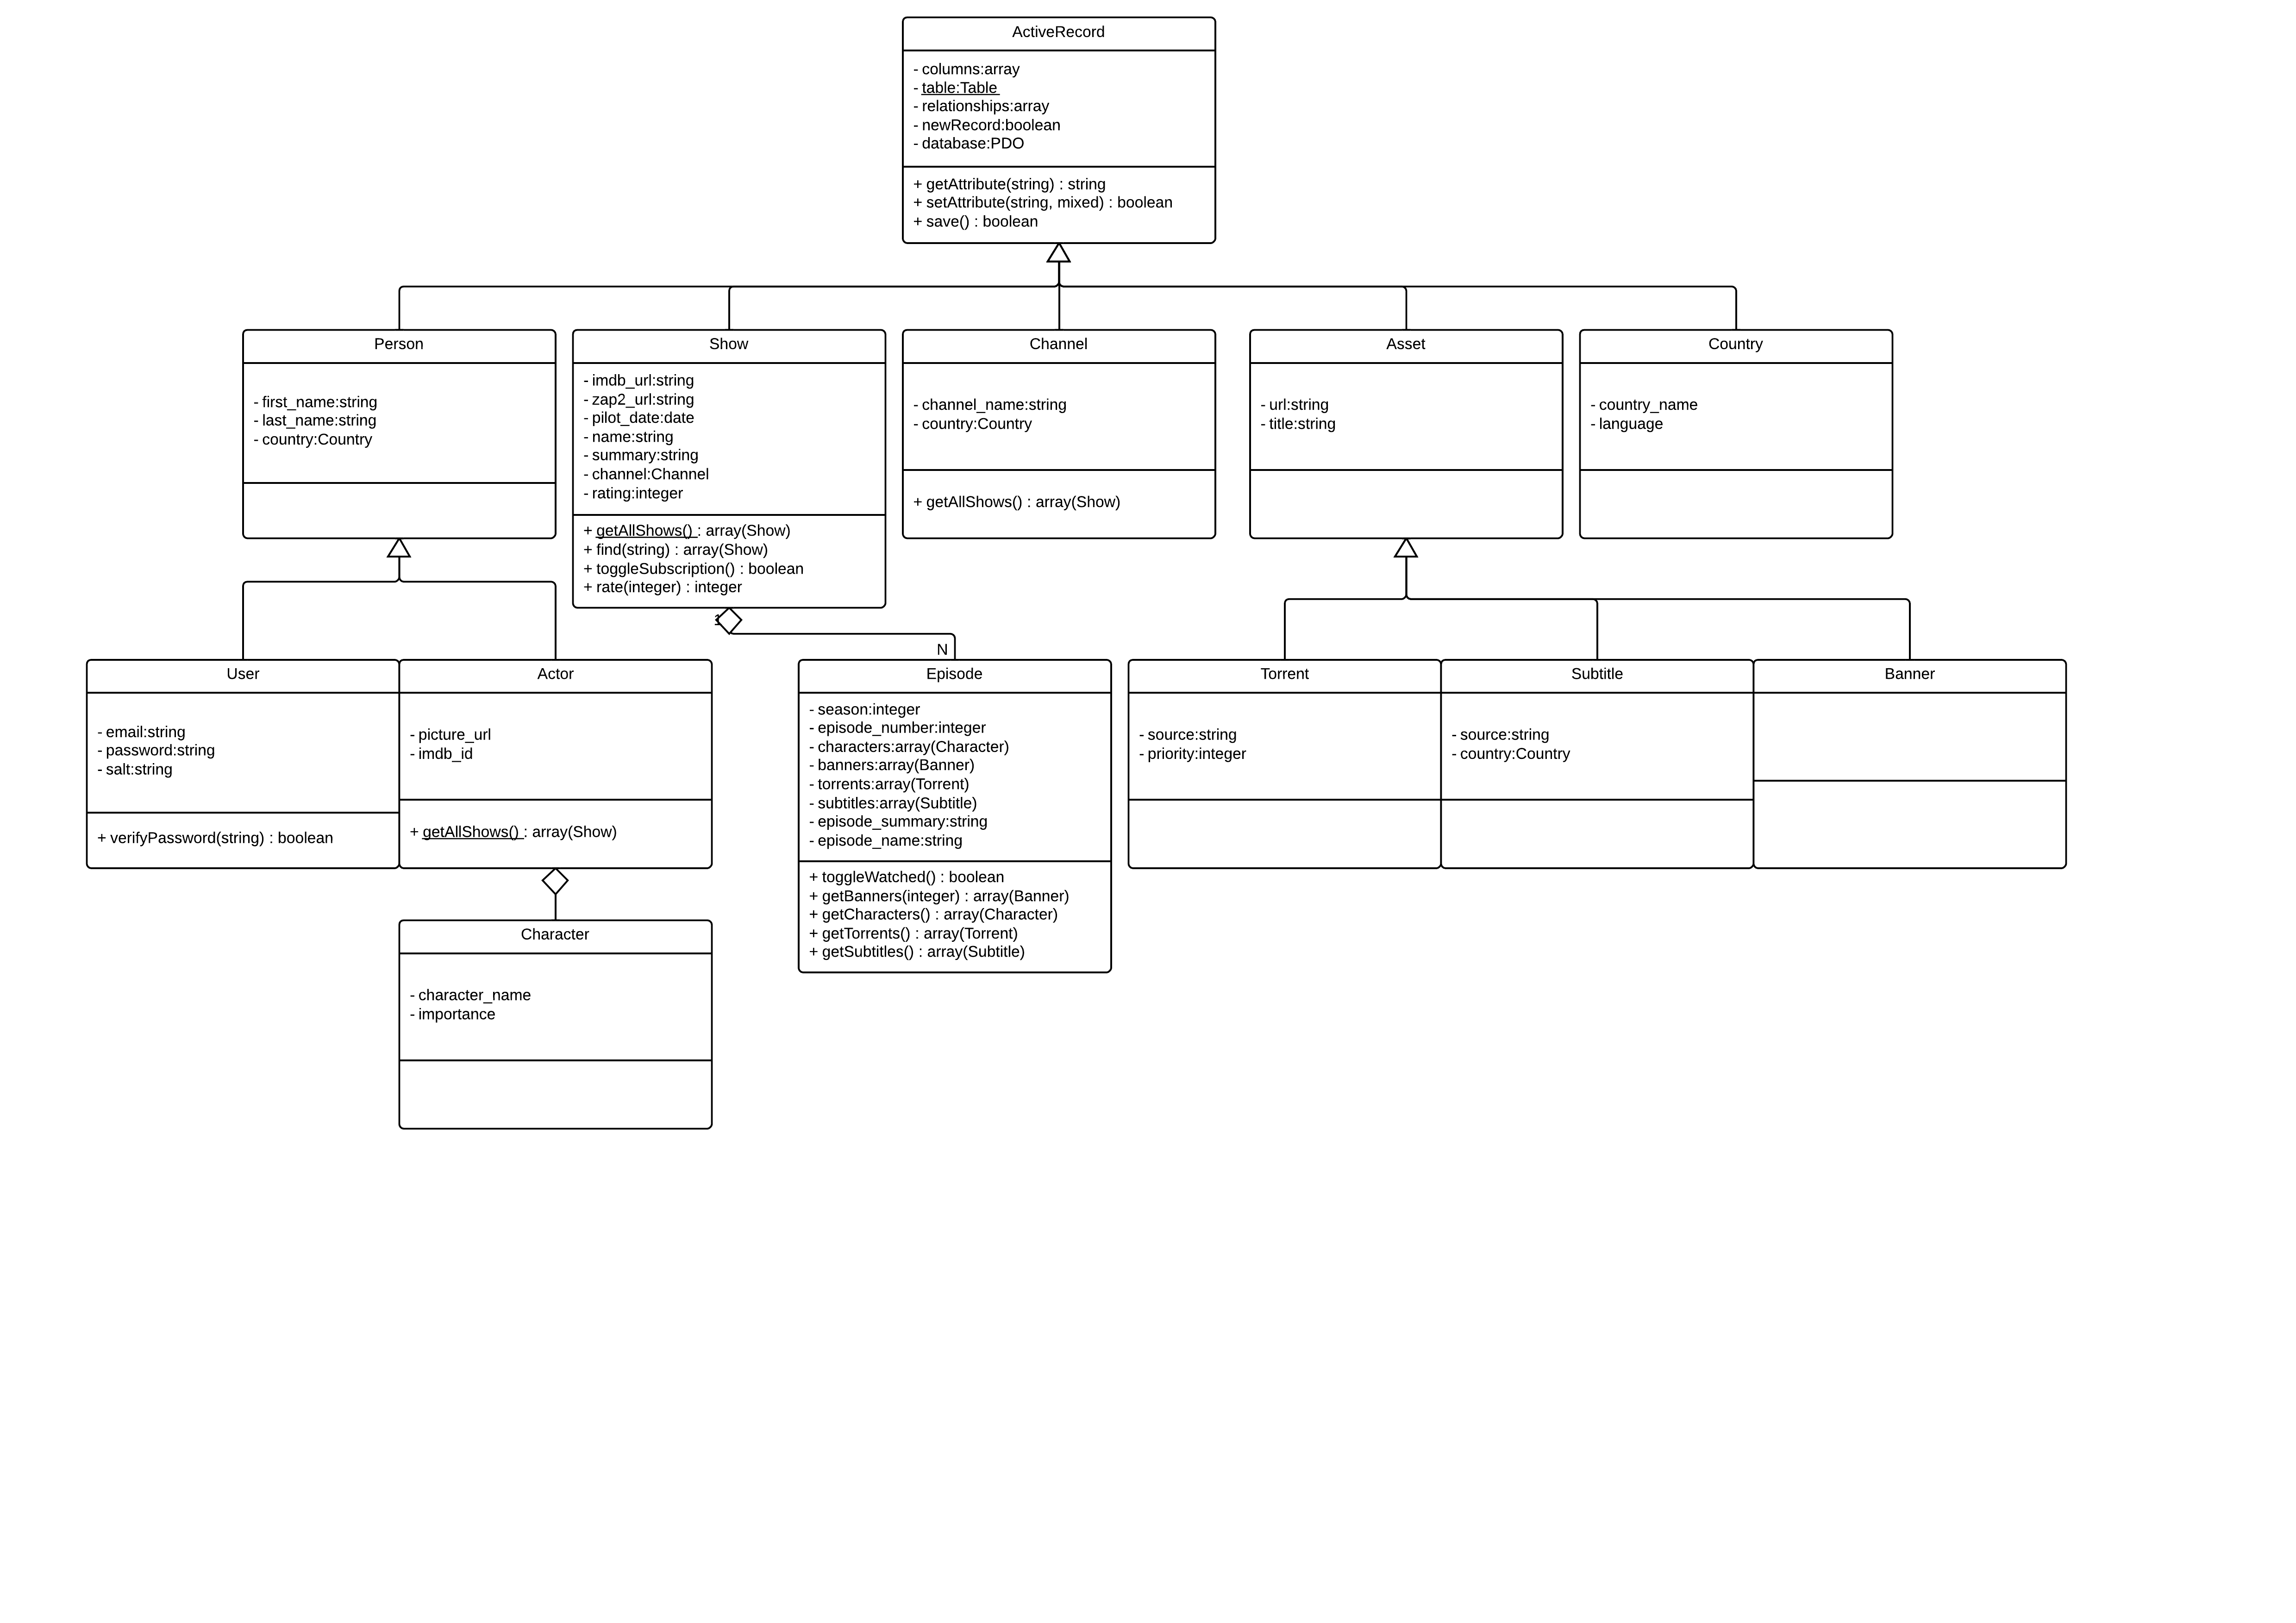
\includegraphics[scale=0.185,angle=90]{graphics/classdiagramnew}}
\caption{Conceptual Class Diagram}
\end{figure}

The conceptual class diagram illustrated above shows the most vital objects for the application and their properties and relationship to one another. Abstract classes, 3rd party library classes or classes utilized by others (such as the database handler class) are intentionally omitted here, but it serves to provide an overview of the relationships between objects within the application.

The most important objects here are \textit{User} and \textit{Show}. The main focus of the system should be on \textit{Show}, because this is the object users will interact the most with. Even without creating a user, it should be possible to browse through the list of shows and their episodes.

However, for more tailored functionality, it's of utmost importance that a \textit{User} is able to log in after being created, and that functionality is provided to allow the user to specify what shows he or she watches.

A \textit{User} may also be an administrator, or any other \textit{Role} with special permissions one may want to assign a user, and it should be possible to create and assign new \textit{Roles} at a later time.

Next, when a \textit{Show} has been selected, it's highly important that we're able to present some information about this \textit{Show}. Information that may be of interest, such as what \textit{Channel} it was originally broadcast on, information about each episode, character, or actor, needs to be retrievable from each \textit{Show} object. 

It's not unlikely that a \textit{User} would like to filter \textit{Shows} by what channel produced or first broadcast it, and as such, it should be possible to retrieve a list of \textit{Shows} from a \textit{Channel} object.

If a \textit{User} has found a \textit{Show} he or she may want to watch, it's very likely that he or she will begin to look for a way to download or stream it. It's therefore desired that lists of \textit{Torrents} and \textit{Subtitles} can be presented for any given \textit{Episode} of any given \textit{Show}.

Furthermore, when a \textit{User} views an \textit{Episode}, he or she may be interested in knowing what \textit{Characters} exist and maybe more importantly, what \textit{Actors} play in this \textit{Episode}, and therefore it's important that a list of \textit{Characters} (sorted by their \textit{importance}) and what \textit{Actors} plays them can be retrieved and presented to the \textit{User}.
\newpage
\subsection{Sequence Diagram}
\begin{figure}[H]

\fbox{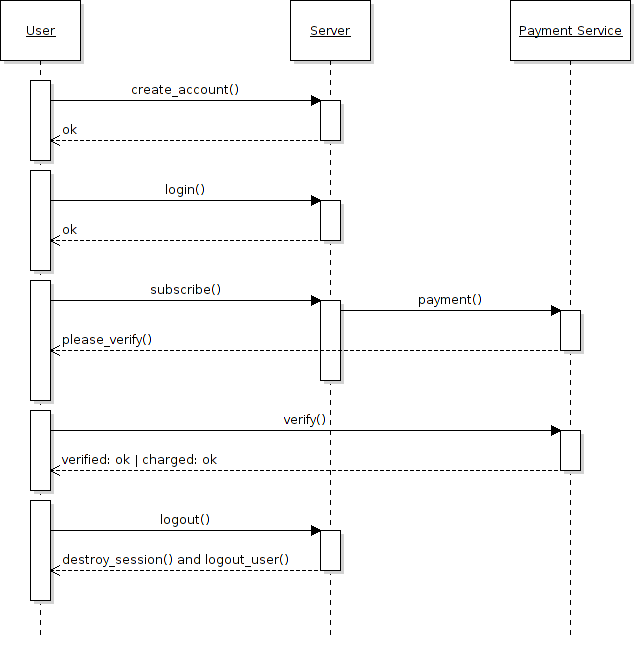
\includegraphics[scale=0.65]{graphics/sequence_diagram}}
\caption{Sequence Diagram (subscription and payment)}
\end{figure}

In order to add a subscription to an user account, the user obviously has to register an account and login to the member-only page.\\
Once this is done the user can request access to a feature which is "pay-to-use" by invoking the subscribe() method.\\
The server will then send a request to the payment service' servers (ie. VISA/Mastercard) and ask them to charge the user a specific amount of money.\\
\\
But before the user is charged, the user has to verify using for example OpenID.
Once this verification process has finalized, the user is charged and sent back to member-only page.\\
\\
The user can then start using the "pay-to-use" functionality or, as shown in the diagram, log out of the application.

%----------------------------------------------------------------------------------------
%	DEL III
%----------------------------------------------------------------------------------------
\newpage
\section{Software Design}
\subsection{Architecture}
We have chosen to do some initial architectural modeling, even though we follow the SCRUM development methodology, which initially does not have an architectural modeling phase. This is because the system that are being developed, could easily end up becoming larger and more complex than initially thought. \\ 
The goal of the initial achitectural modeling is not to write tons of documentation and end up with a final plan, but rather to identify and agree on an architectural and technical  strategy within the development team. The architectural model will be more complex and detailed later during development. \\
By performing some high-level architectural modeling at the beginning of the project, we hope to improve alot of other factors throughout the project. \cite{agilemodeling}

\begin{itemize}
	\item This will allow us to think about some of the more critical issues we will be facing, and potentially avoid spending time on something that woud prove later to be impossible, because of this we will most likely get \textbf{improved productivity}
	\item The project will be at a \textbf{reduced technical risk} bacuse the team would have some sort of vision on how to solve problems before encountering them. 
	\item \textbf{Development time} will also hopefully be reduced, given that better decisions and estimates could be taken.
	\item The high-level architecture models will \textbf{improve communication} within the team because it helps with sharing thoughts on how to solve problems.
	\item This will also \textbf{improve team organization} because it will make it easier to delegate tasks between each SCRUM sprint.
\end{itemize}

Bacuse of our development method we have to be careful not to spend too much time on the initial achitectural modeling. The amount of value we get from doing the modeling drasticly drops if we oversaturate the model.\\
Figure 4. shows a graphical representation of the value of initial architectural modeling over time.
\begin{figure}[H]
\fbox{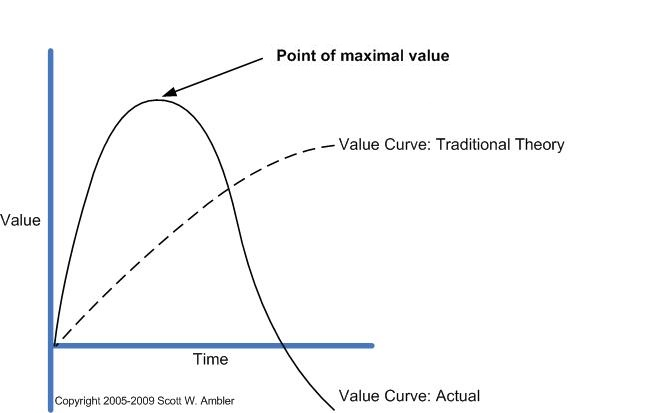
\includegraphics[scale=0.8]{graphics/valueOfModeling}}
\caption{Value of modeling \cite{valueofmodeling}}
\end{figure}

Since we are not locked to a certain method of doing architectural modeling, we have chosen to only model a user interface flow chart, a UML deployment diagram and a technology stack diagram. We believe these models will help the team the most without spending too much time modeling.

% Client-Server backend: REST Web-services for compatibility with default EmberJS API 
% Model-View-Whatever frontend: EmberJS presents data with views determined by controllers through user interaction (i.e clicking a link sends the "action" (what link was clicked) for processing by the controller, which loads data from the model and sends it to the appropriate view for rendering)
\subsection{Architectural Models}
\subsubsection{UML Deployment Diagram}
In order to ensure good performance and a stable system, the hardware is divided into two layers, internal and external.
The components of the internal system is hosted and maintained by FrostByte, whereas the components of the external system is run by two 3rd parties (ie Visa/Mastercard and TVDB).
\\
Following the diagram is a more in depth explanation of the different components.
\begin{figure}[H]
\fbox{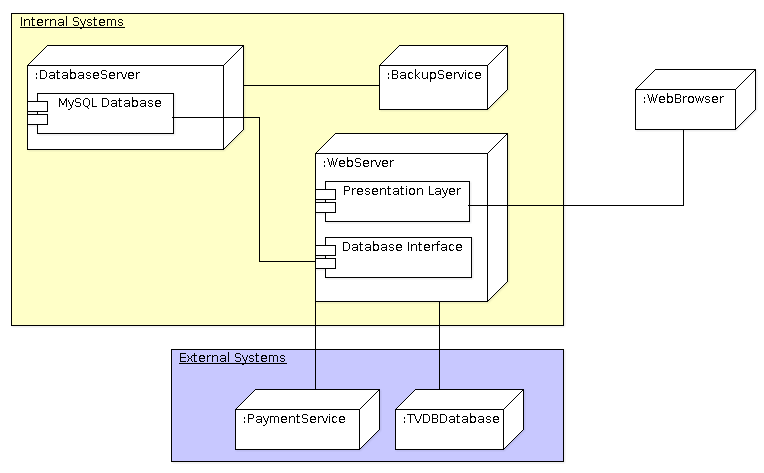
\includegraphics[scale=0.5]{graphics/deployment.png}}
\caption{Deployment Diagram}
\end{figure}

\paragraph*{WebBrowser}~\\
By WebBrowser we are generally talking about the clients, i.e. the users of EpisodeGuide. The clients use a web browser to access data stored on EpisodeGuide through HTTP requests.\\
Supported browsers include Mozilla Firefox, Opera, Chrome and Internet Explorer.

\paragraph*{DatabaseServer}~\\
The database server(s) will store all the available data, including user details, episode information and information about actors. EpisodeGuide will use a graph-oriented database~\cite{website:graphdb}, i.e. a database that uses graph theory to store, map and query relationships. The reason for this is that EpisodeGuide have a lot of data that is linked together, and this could potentialy cause a problem with performance if relational databases and JOIN operations have been used instead.

\paragraph*{WebServer}~\\
The webserver will handle the delivery of data to the clients. Here we have two different components, i.e. the presentation layer and a database interface.\\
The presentation layer provide a way for clients to watch and interact with the content.\\
The database interface is handling the connection(s) to the database(s) and provide a way for the backend to save, modify and delete content.\\
For the database software EpisodeGuide will use the open source NGiNX webserver.

\paragraph*{BackupService}~\\
As a backup service EpisodeGuide will use an encrypted server leveraging the power of RAID-5 with parity bits. Raid-5 will provide a good way to ensure that data is backed up in a safe manner.\\
If a hard drive in this server dies, the use of parity bits will ensure that the lost data can be restored and thus ensuring that no data is lost.\\
Since the database also store information about the clients (i.e. users) the content is fully encrypted using the AES encryption algorithm.

\paragraph*{PaymentService}~\\
\textit{Since this is a 3rd party service, EpisodeGuide has little to no information about the different components or how they are organized.}

\paragraph*{TVDBDatabase}~\\
\textit{Since this is a 3rd party service, EpisodeGuide has little to no information about the different components or how they are organized.}

\subsubsection{User interface flow chart}
\begin{figure}[H]
\fbox{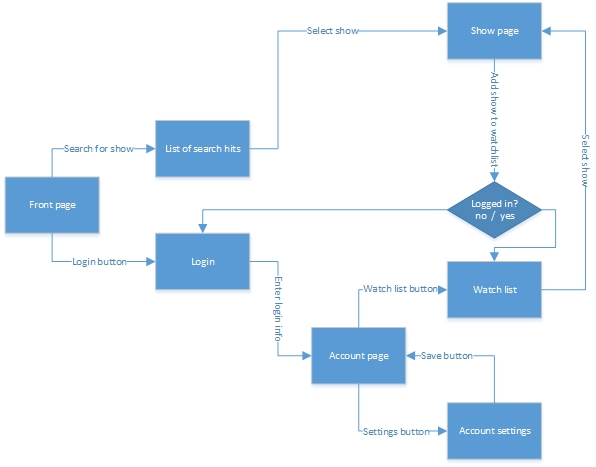
\includegraphics{graphics/UIworkflow}}
\caption{UI flow chart}
\end{figure}

The user interface flow chart is a rough model of the primary functions of the system, and how the end user will navigate through the system. Most of the functions are not modelled and will be implemented around the key features that are modelled. 

\subsection{Back-end}
An application that works with such large amounts of data as EpisodeGuide, where data is also structured in a hierarchy (Channel \guillemotright Show \guillemotright Episode), calls for a database -- one that easily identifies relationships between entries, is fast to search through, and scales well since the amount of data starts out big and only keeps growing. 

As any site that expects large volumes of traffic, reliability is highly important, and thus a quick web server running on a reliable operating system is required. When it comes to the application itself, it should be easily extensible in the future without requiring massive modification to the codebase. As such, modularity is important and therefore separation of components should be clear, and the back-end separate from the front-end. This is also the reason the back-end is separate from the front-end in this report.  


%%
%% CentOS
%% MariaDB
%% Nginx
%% REST

\subsubsection{Platform}
With stability as a priority for the server operating system, Linux or FreeBSD seems like natural candidates, but as Linux is more commonly used by developers and thus more commonly supported, it becomes a natural choice. Determining the right distribution for a site that will be taking payments, security plays a huge role. Whereas Debian has a lot more packages in its package managing system and supports upgrading from one version to the next smoothly, CentOS comes with 10 years support and security patches, and generally has great support from vendors in the enterprise world what with it being a RHEL derivative. A major disadvantage of using CentOS over Debian is the lower amount of packages in its repositories, but this disadvantage pales in comparison to the benefits of a lengthy lifespan.
 
\subsubsection{Database}
When the application being developed is supposed to work with large sets of data that is interconnected -- where a TV show contains a set of episodes, which in turn contains a list of characters played by different actors, who in turn play other characters in other episodes of other TV shows -- one quickly realizes that a relational database may scale poorly.
Instead, a graph database like Neo4j seems like a prominent candidate. Neo4j is one of the most popular graph databases today, and thus provides good support and documentation. Neo4j comes with a RESTful API, for which there also exists a PHP wrapper allowing which allows the application to be written in PHP, and whilst the front-end (as further explained in the front-end section) by default communicates with a RESTful API, writing the back-end as a middleware in PHP allows for future changes without having to modify the front-end code. Should the database system be changed in the future, the same queries can still be made from the front-end to retrieve data from the back-end.
By using a graph database, we have the advantages of faster searches through large sets of data -- especially when it comes to depth searching, such as creating recommendations or finding what other TV-shows a character's actor has been in. 

\subsubsection{Web Server}
Apache has ruled the kingdom of web servers for a very long time, but in recent years, this king has been overthrown by competitors such as nginx, cherokee and lighttpd. Nginx provides very simple and highly modular configuration which follows CSS-like syntax, which makes configuration a breeze; and whilst lighttpd has a very low memory footprint in comparison to Apache, nginx still excels in benchmarks. For this reason, nginx has been chosen as the best web server for this project.

\subsubsection{Web services and design pattern}
The application as a whole follows a client-server design pattern, in that a front-end is a client communicating with the backend (server). This means that creating an app for a phone, tablet, or any other device really is just creating yet another front-end, and the front-end on the website really is just a front-end client hosted on the same server, which makes the system very flexible.

The back-end should mainly operate through an API, parts of which should be open to the public. Modifications to the catalogue of TV shows should not be allowed by users with insufficient permissions, but finding and reading data should of course be available to anybody. For optimal flexibility and compatibility with potential future extensions either by the development team or by independent app developers, a RESTful API should be developed.
A major advantage of using a RESTful API is that it fits perfectly with the HTTP protocols different states: PUT (update), POST (create), GET (read) and DELETE (remove), which lets the action be defined by the HTTP method. 
SOAP and REST both have benefits, but REST is very simple to work with without requiring a special library or plugin.  

\subsection{Front-end}
Web sites are conventionally made using the standard languages provided for it: HTML, CSS, and JavaScript. However, it's becoming increasingly popular to instead work with abstractions of these in the form of frameworks or languages that is parsed or compile into native javascript or CSS for various reasons. With native applications, running as standalone programs on a computer, we have frameworks such as .NET to speed up development by letting developers spend more time on solving \textit{relevant} problems for the application, instead of solving \textit{trivial} problems (such as string or data processing).

Today, a lot of applications are moving more and more to the web, but the basic concept is very similar: Code is downloaded and run locally, and displays information retrieved over the web. The main difference is that with web application, code runs in a sandbox (the web browser). Therefore, we have taken a look at various front-end frameworks for developing web applications almost on par with native applications, without wasting time on reinventing the wheel.   

\subsubsection{Design pattern}

MVC has become more or less a standard way of decomposing web applications into different components (models, views and controllers), which makes it easy to modify or add new components of either type independently. Because the application has a lot of data that is simply presented in different ways (listing of episodes, shows, and so on), it seems logical to use a framework that makes use of this design pattern.

\subsubsection{Technology}
After comparing two of the most prominent javascript frameworks, Angular and Ember, it was found that Angular's \textit{dirty checking} leads to less than optimal performance when the DOM containes a large amount of elements, an issue not present in Ember. Since the application will be working with large sets of data in the form of TV shows, displaying an ever increasing list of shows, and thus may have a huge amount of elements in the DOM, this is a requirement Ember can satisfy.

Ember takes inspiration from already mature open source technology before it -- such as Backbone.js and Ruby on Rails -- and uses the familiar terminology of Models, Views and Controllers, whereas Angular introduces concepts such as directives, scopes and transclusion, which makes Ember faster to get started with than Angular.

Furthermore, for the web application to be easily extensible with e.g mobile apps or 3rd party apps, it would make sense for the back-end to provide an API in the form of web services. Not only is this useful for mobile apps or 3rd party apps, but it's how Ember works with data by default: It works with data retrieved from RESTful web services, and this in turn helps separating the front-end from the back-end while also allowing the front-end to run on a completely different server, should this be needed in the future. 

Separating the front-end and the back-end allows for different software architectures for the front-end and the back-end, and allows them to be developed independently. It lets the front-end operate as a client retrieving and modifying sets of data from the server via the API, just as any other form of client would.

Ember uses RequireJS, which makes development modular by allowing code to be written as packages and included as needed -- a feature that goes hand in hand with the SCRUM development methodology. Each package provides a list of dependencies, as does the application itself, so including the correct version and in the right order can be done automatically, and different releases can depend on different version of packages. Additionally, \textit{views} can be displayed with different \textit{templates} as Ember fully supports and promotes Handlebars for templating, which makes displaying the same data in different forms rather easy.

One of the key advantages of Ember is data binding. Data binding means that when a property present in multiple object changes in one object, it's also updated in other objects. Another advantage is state-management (is a user logged in or out?), and auto-updating of templates when the underlying data changes. For example, when a user decides to \textit{subscribe} to a TV show, any other elements listing shows the user has subscribed to would be updated with the new subscription. 
\input{Design/architecture.tex}


%----------------------------------------------------------------------------------------
%	BIBLIOGRAPHY (References)
%----------------------------------------------------------------------------------------
\newpage
\bibliographystyle{plain}
\bibliography{references}

%\bibliographystyle{unsrt}
%\bibliography{Sources}
%\begin{thebibliography}{99} % Bibliography - this is intentionally simple in this template

%\bibitem[Figueredo and Wolf, 2009]{Figueredo:2009dg}
%Figueredo, A.~J. and Wolf, P. S.~A. (2009).
%\newblock Assortative pairing and life history strategy - a cross-cultural
%  study.
%\newblock {\em Human Nature}, 20:317--330.
 
%\end{thebibliography}

%----------------------------------------------------------------------------------------------------------------------------------------------------
\end{document}